\documentclass{article}

\usepackage{graphicx}
\usepackage{tikz}
\usepackage{tikzsymbols}
\usetikzlibrary{calc,patterns,shapes.geometric}
\pagestyle{empty}
\usepackage[margin=0pt]{geometry}
\geometry{papersize={14in,12in}}

\def\centerarc[#1](#2)(#3:#4:#5){\draw[#1] ($(#2)+({#5*cos(#3)},{#5*sin(#3)})$) arc (#3:#4:#5);}

\begin{document}
	\begin{figure}
		\centering
		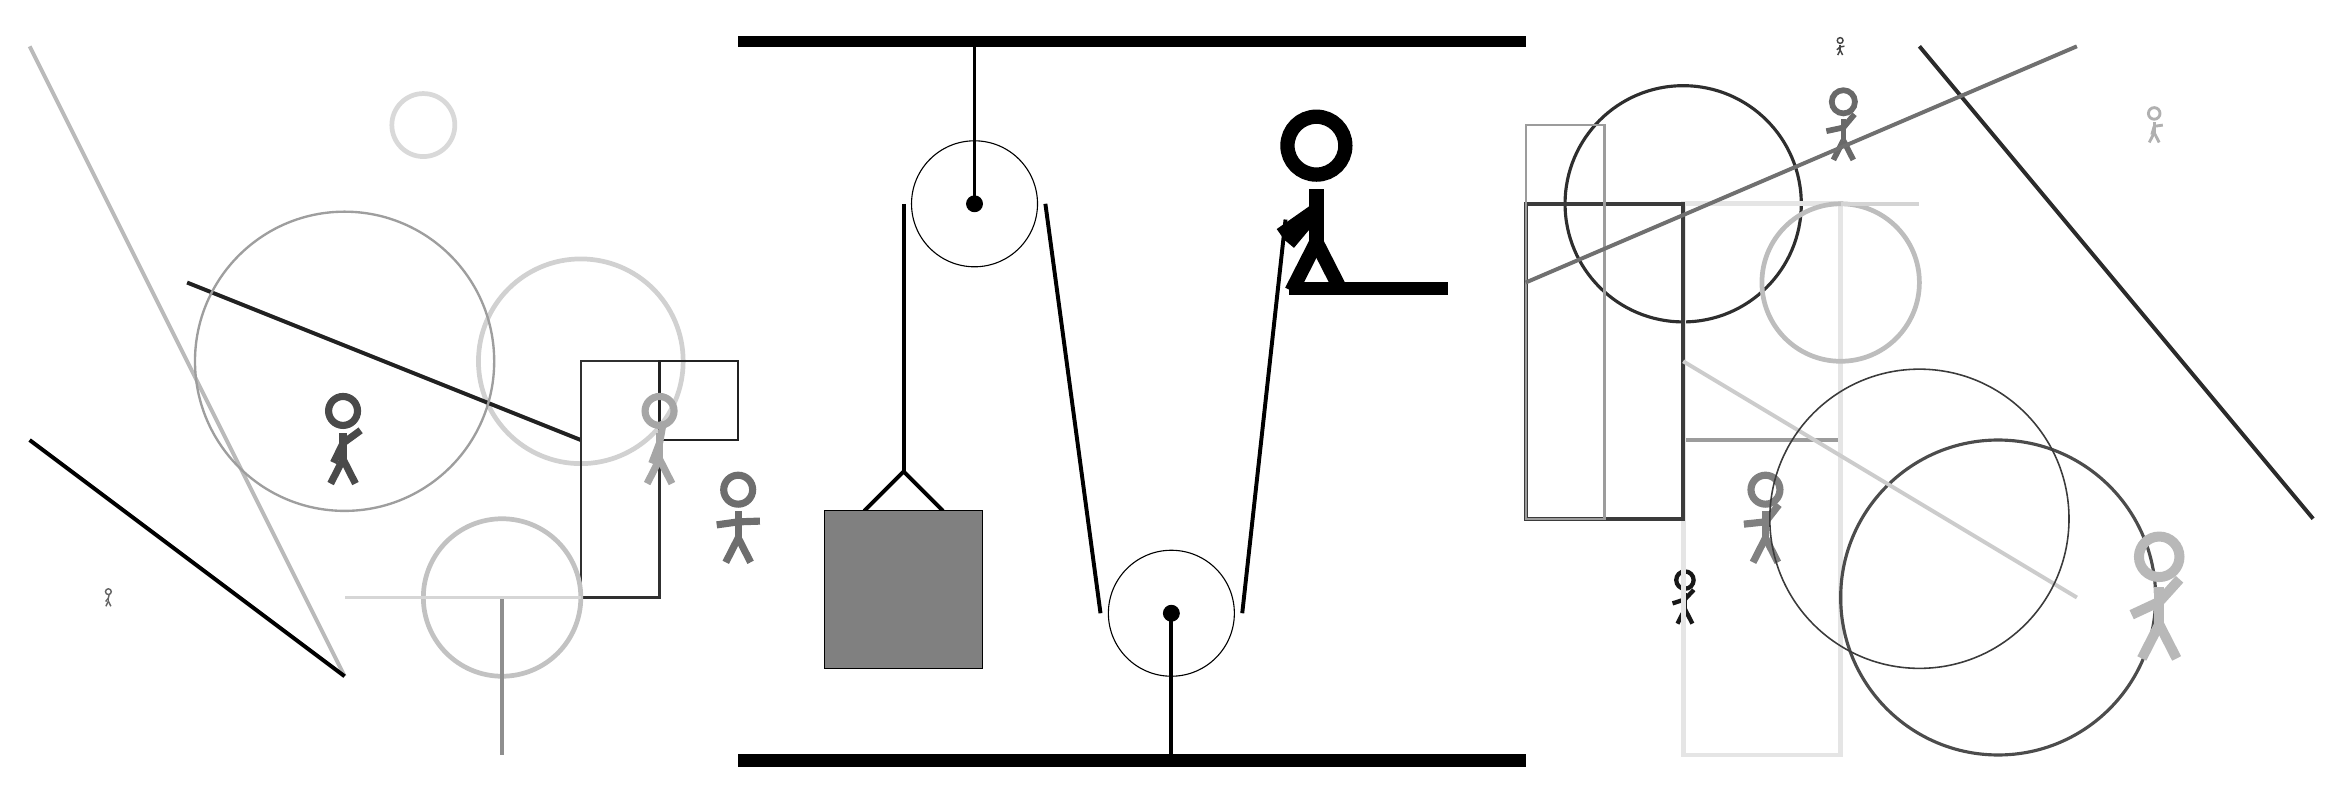
\begin{tikzpicture}
			%%%%% START %%%%%
			
			\draw[fill=black] (-2, 9) rectangle (8, 9.125);
			
			\draw [line width=0.6mm, color=black!18](-4, 5) circle (1.3);
			
			\node[line width=0.2mm, color=black!31] at (16, 8) {\Strichmaxerl[2][74][8]};
			\node[line width=0.4mm, color=black!57] at (-2, 3) {\Strichmaxerl[5][8][2]};
			\node[line width=0.5mm, color=black!59] at (12, 8) {\Strichmaxerl[4][12][50]};
			
			\draw[line width=0.5mm, color=black!87](-4, 4) -- (-9, 6);
			
			\node[line width=0.2mm, color=black!50] at (11, 3) {\Strichmaxerl[5][6][52]};
			
			\draw[line width=0.3mm, color=black!81] (-4, 5) rectangle (-3, 2);
			\draw[line width=0.5mm, color=black!27](-7, 1) -- (-11, 9);
			\node[line width=0.5mm, color=black!91] at (10, 2) {\Strichmaxerl[3][18][47]};
			\draw[line width=0.5mm, color=black!83](13, 9) -- (18, 3);
			\draw [line width=0.6mm, color=black!24](-5, 2) circle (1.0);
			\node[line width=0.7mm, color=black!71] at (-7, 4) {\Strichmaxerl[5][64][36]};
			\draw [line width=0.4mm, color=black!82](10, 7) circle (1.5);
			
			\node[line width=0.6mm, color=black!61] at (-10, 2) {\Strichmaxerl[1][51][78]};
			\draw[line width=0.5mm, color=black!39] (10, 0) rectangle (12, 4);
			\draw[line width=0.6mm, color=black!10] (10, 0) rectangle (12, 7);
			
			\draw[line width=0.5mm, color=black!44](-5, 0) -- (-5, 2);
			\draw[line width=0.5mm, color=black!77] (10, 7) rectangle (8, 3);
			\node[line width=0.4mm, color=black!73] at (12, 9) {\Strichmaxerl[1][41][10]};
			\draw [line width=0.6mm, color=black!26](12, 6) circle (1.0);
			\draw [line width=0.4mm, color=black!70](14, 2) circle (2.0);
			
			\draw[line width=0.3mm, color=black!39] (8, 8) rectangle (9, 3);
			\draw [line width=0.3mm, color=black!38](-7, 5) circle (1.9);
			\draw[line width=0.5mm, color=black!100](-7, 1) -- (-11, 4);
			\draw[line width=0.5mm, color=black!17](12, 7) -- (13, 7);
			
			\node[line width=0.6mm, color=black!28] at (16, 2) {\Strichmaxerl[7][25][48]};
			
			\draw [line width=0.6mm, color=black!15](-6, 8) circle (0.4);
			\draw[line width=0.3mm, color=black!87] (-3, 4) rectangle (-2, 5);
			
			\draw[line width=0.5mm, color=black!56](8, 6) -- (15, 9);
			\draw[line width=0.5mm, color=black!20](10, 5) -- (15, 2);
			\node[line width=0.7mm, color=black!35] at (-3, 4) {\Strichmaxerl[5][69][80]};
			
			\draw [line width=0.2mm, color=black!77](13, 3) circle (1.9);
			\draw[line width=0.5mm, color=black!16](-4, 2) -- (-7, 2);
			
			
			\draw (3.5, 1.8) circle (0.8);
			\draw[fill=black] (3.5, 1.8) circle (0.1);
			\draw[line width=0.5mm] (3.5, 1.8) -- (3.5, 0);
			
			\draw (1, 7) circle (0.8);
			\draw[fill=black] (1, 7) circle (0.1);
			\draw[line width=0.5mm] (1, 9) -- (1, 7);
			
			\draw[line width=0.5mm](-0.4, 3.1) --  (0.1, 3.6) -- (0.6, 3.1);
			\draw[fill=black!50] (-0.9, 3.1) rectangle (1.1, 1.1);
			
			\draw[line width=0.5mm](0.1, 7) -- (0.1, 3.6);
			\centerarc[line width=0.5mm](1, 7)(180:0:0.9)
			\draw[line width=0.5mm](1.9, 7) -- (2.6, 1.8);
			\centerarc[line width=0.5mm](3.5, 1.8)(180:360:0.9)
			\draw[line width=0.5mm](4.4, 1.8) -- (4.95, 6.8);
			
			\node at (5.3, 7) {\Strichmaxerl[10][35][-130]};
			\draw[fill=black] (5, 6) rectangle (7, 5.85);
			
			\draw[fill=black] (-2, 0) rectangle (8, -0.15);
			
			%%%%% END %%%%%
		\end{tikzpicture}
	\end{figure}	
\end{document}